\documentclass[12pt]{article}

\usepackage{bm}
\usepackage{amsmath}
\usepackage{amssymb}
\usepackage{cite}
\usepackage{indentfirst}
\usepackage{url}
\usepackage{graphicx}

\title{Homework 1 \\\vspace{1em}
\large CS 525: Deep Learning}
\author{
  Jerry Duncan \\
  jdunca51@vols.utk.edu
}
\date{February 23, 2020}
\begin{document}
\maketitle
\pagebreak

\section{Problem 1}

\subsection{Output}

The net for a a simple perceptron is $w \cdot x + b$.
In this case that's equivalent to $w_1x_1 + w_2x_2 + b = y$ or $0.2*2 + 0.3*1 + 0.1 = 0.8$.
Then we pass the net to the sigmoid function to get the output.
The answer is then $y = sigmoid(0.8) = 0.68997$.

\subsection{Loss}

Binary Cross-Entropy is defined by the following formula:

$$
E = - \frac{1}{N} \sum_{i=1}^{N} y_i * log(\hat{y_i}) + (1 - y_i) \cdot log(1 - \hat{y_i})
$$

When we plug in our values from above, $\hat{y} = 0.68997$ and $y = 1$,
the right side of the equation simplifies to zero and we're left with the following:

$$
E = - \frac{1}{1} 1 * log(0.68997) = -log(0.68997) = 0.3711
$$

Therefore, the answer is $E = 0.3711$.

\subsection{Bias}

A perceptron on its own is able to learn any linear function that goes through the origin.
The issue is that not all useful functions go through the origin.
A bias acts like a y-intercept in that regard, allowing the perceptron to learn a wider variety of functions
 and solve more problems.
It can allow the perceptron to better learn a split through the dataset that
 a linear combination of the inputs might not be able to learn.

\section{Problem 2}

The number of channels in the output is always equal to the number of kernels
 in that layer.

\subsection{Output}

$$
Out =
\begin{bmatrix}
  1 & 1 & 1 \\
  0 & 1 & 3 \\
  0 & 0 & 1
\end{bmatrix}
$$

The output would have a shape of (3, 3, 1).
(width, height, number of kernels).

\subsection{Two Channel Input \& Output}

$$
Out =
\begin{bmatrix}
  2 & 2 & 2 \\
  0 & 2 & 6 \\
  0 & 0 & 2
\end{bmatrix}
$$

The output would have a shape of (3, 3, 1).
(width, height, number of kernels).

\subsection{Two Kernel Output}

The first kernel's output is channel 1 of the output.

$$
Out_1 =
\begin{bmatrix}
  1 & 1 & 1 \\
  0 & 1 & 3 \\
  0 & 0 & 1
\end{bmatrix}
$$

The second kernel's output is channel 2 of the output.

$$
Out_2 =
\begin{bmatrix}
  1 & 1 & 1 \\
  0 & 1 & 3 \\
  0 & 0 & 1
\end{bmatrix}
$$

The output would have a shape of (3, 3, 2).
(width, height, number of kernels).

\section{Problem 3}

\subsection{Layer 1 - Convolution Layer}

The output dimensions are $((\frac{w_i - w_f}{s} + 1), (\frac{h_i - h_f}{s} + 1), \# filters)$.
In our case, $w_i = 21, w_f = 5, h_i = 21, h_f = 5, s = 2, \# filters = 6$.
That means the output dimensions are:

$$
((\frac{21 - 5}{2} + 1), (\frac{21 - 5}{2} + 1), 6) =
$$
$$
= (9, 9, 6)
$$

Weights are calculated by $(w_f * h_f * input\_depth) * \# filters$
In our case, $w_f = 5, h_f = 5, input\_depth = 3, \# filters = 6$.
That means the number of weights is:

$$
(5 * 5 * 3) * 6 = 76 * 6 = 450
$$

There is one bias for each kernel in the layer, of which there are 6 so there are 6 biases.

\subsection{Layer 2 - Max Pooling Layer}

Input shape = $(9, 9, 6)$.

The output dimensions are $((\frac{w_i - w_f}{s} + 1), (\frac{h_i - h_f}{s} + 1), input\_depth)$.
In our case, $w_i = 9, w_f = 3, h_i = 9, h_f = 3, s = 2, input\_depth = 6$.
That means the output dimensions are:
$$
((\frac{9 - 3}{2} + 1), (\frac{9 - 3}{2} + 1), 6) =
$$
$$
= (4, 4, 6)
$$

There are no weights or biases for a Max Pooling Layer.

\subsection{Layer 3 - Convolution Layer}

Because the padding is the same, our output width and height will be the same, but the depth will
 be equal to the number of filters in this layer (10).

That means the output dimensions are:

$$
= (4, 4, 10)
$$


Weights are calculated by $(w_f * h_f * input\_depth) * \# filters$
In our case, $w_f = 3, h_f = 3, input\_depth = 6, \# filters = 10$.
That means the number of trainable parameters is:

$$
(3 * 3 * 6) * 10 = 54 * 10 = 540
$$

There is one bias for each kernel in the layer, of which there are 10 so there are 10 biases.


\subsection{Layer 4 - Flatten Layer}

Input shape = $(4, 4, 10)$.

The output dimensions are $\Pi_{i=0}^{N} input\_shape_i$.

In our case, $input\_shape_0 = 4, input\_shape_1 = 4, input\_shape_2 = 10$.
That means the output dimensions are:
$$
 4 * 4 * 10
$$
$$
= 160
$$

There are no weights or biases for a Flatten Layer.


\subsection{Layer 5 - Dense Layer}

Input shape = $(160,)$

The output shape is equal to the number of neurons in the layer.
In this case there are 10 so the output shape is $(10,)$.

There are $input\_shape$ weights for each neuron in the layer.
That means there are $160 * 10 = 1600$ weights.

There is one bias for each neuron in a dense layer, of which there are 10 so there are 10 biases.


\section{Problem 4}

\subsection{Learning Rates}

Answers found in Figure \ref{fig:error}.

\begin{figure}[!htb]
  \centering
  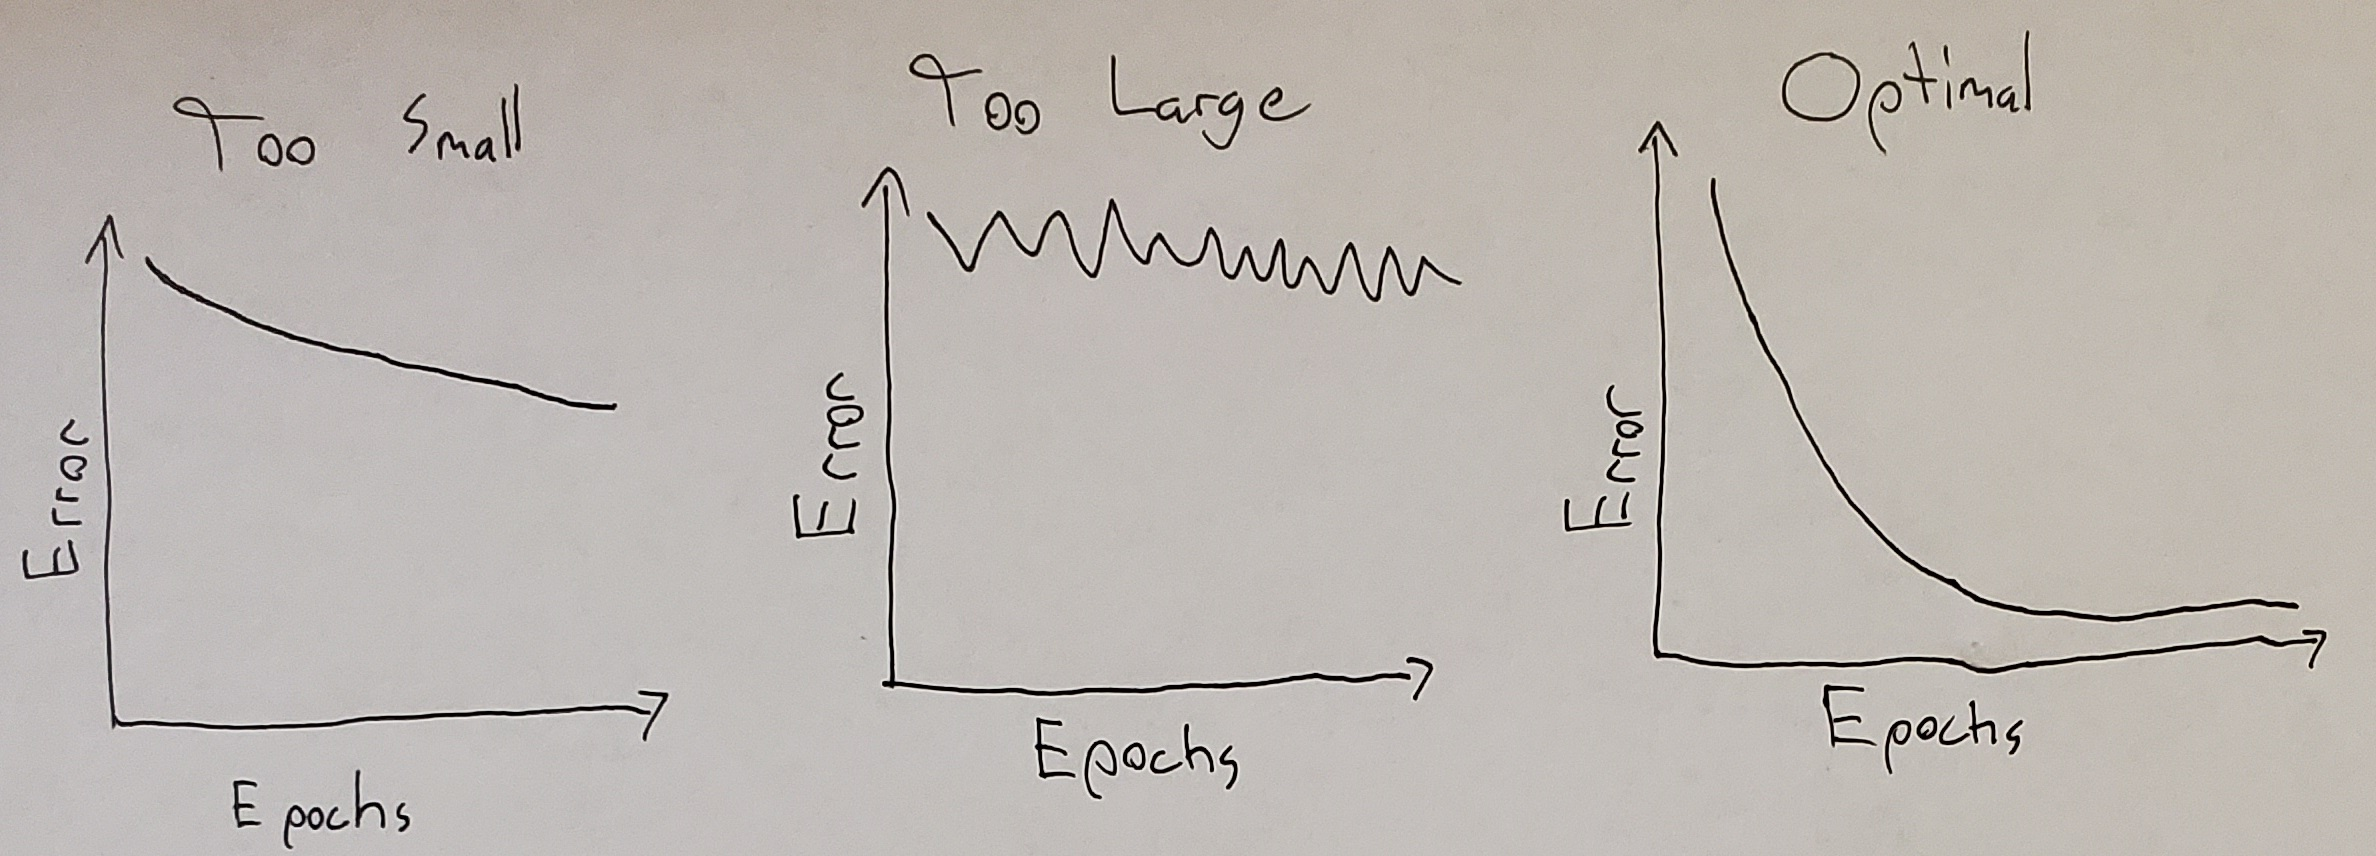
\includegraphics[width=\textwidth]{error.jpg}
  \caption{Error vs Learning Rate}
  \label{fig:error}
\end{figure}


\subsection{Stochastic Gradient Descent}

The first reason is that SGD does each sample individually, albeit a random sample.
The problem with this is that it's still just as expensive as gradient descent in terms
 of sheer computation per epoch.
We can alleviate this by doing computation in random mini-batches instead.
Typically we can calculate gradients this way for little to no additional
 computational cost over doing it for an individual sample, so it saves us
 a considerable amount of computation and still works well enough at
 getting to the minimum.

The second reason is that as SGD get closer to a minimum, it may have a hard
 time finding the minimum because the learning rate is still high and
 the gradient update may cause it to overshoot the minimum at each iteration.
This can cause the model to need to run for a considerably longer time than
 necessary to get to the minimum.
The way to fix this is by annealing the learning rate over time -- that is,
 slowly lowering it so that as we presumably get closer to the minimum,
 we prevent ourselves from overshooting it.

\section{Problem 5}

\subsection{Output Weight Update}

The weight update for weight i is $w_i^f = w_i^f - \alpha \frac{\partial E_{total}}{\partial w_i^f}$
where
$$
\frac{\partial E_{total}}{\partial w_i^f} = \delta_i^f * \frac{\partial net_i}{\partial w_i^f}
$$
$$
\delta_i^f = \frac{\partial E_{total}}{\partial o_i(X)} * \frac{\partial o_i(X)}{\partial net_i}
$$

\subsection{Output Bias Update}

The update to the bias for neuron i is $bias_i^f = bias_i^f - \alpha \delta_i^f$.

\subsection{Conv. Weight Update}

The update to weight i is $w_i^c = w_i^c - \alpha \delta_i^c \circledast X_i$ where
$$
\delta_i^c = \delta_i^f * w_i^f * \frac{\partial o_i(X)}{\partial net_i}
$$
$$
\delta_i^f = \frac{\partial E_{total}}{\partial o_i(X)} * \frac{\partial o_i(X)}{\partial net_i}
$$

\subsection{Conv. Bias Update}

The update to the biases of a convolutional layer are equal to the sum of the deltas for each channel.

$$
bias_i^c = bias_i^c - \alpha \sum_j^N \delta_j^c
$$

\bibliographystyle{abbrv}

\end{document}